\documentclass[]{extarticle}
\usepackage[T1]{fontenc}
%\usepackage{ebgaramond}
%\usepackage{LibreBodoni}
\usepackage{librecaslon}
\usepackage[a5paper]{geometry}
\usepackage{tikz}
\usetikzlibrary{positioning}
\pagestyle{empty}

%\fontfamily{LibreBodoni-TLF}\selectfont

\definecolor{dpurple}{HTML}{800080}

\begin{document}
\begin{tikzpicture}[remember picture,overlay]
	% draw image
	\node[inner sep=0] at (current page.center) {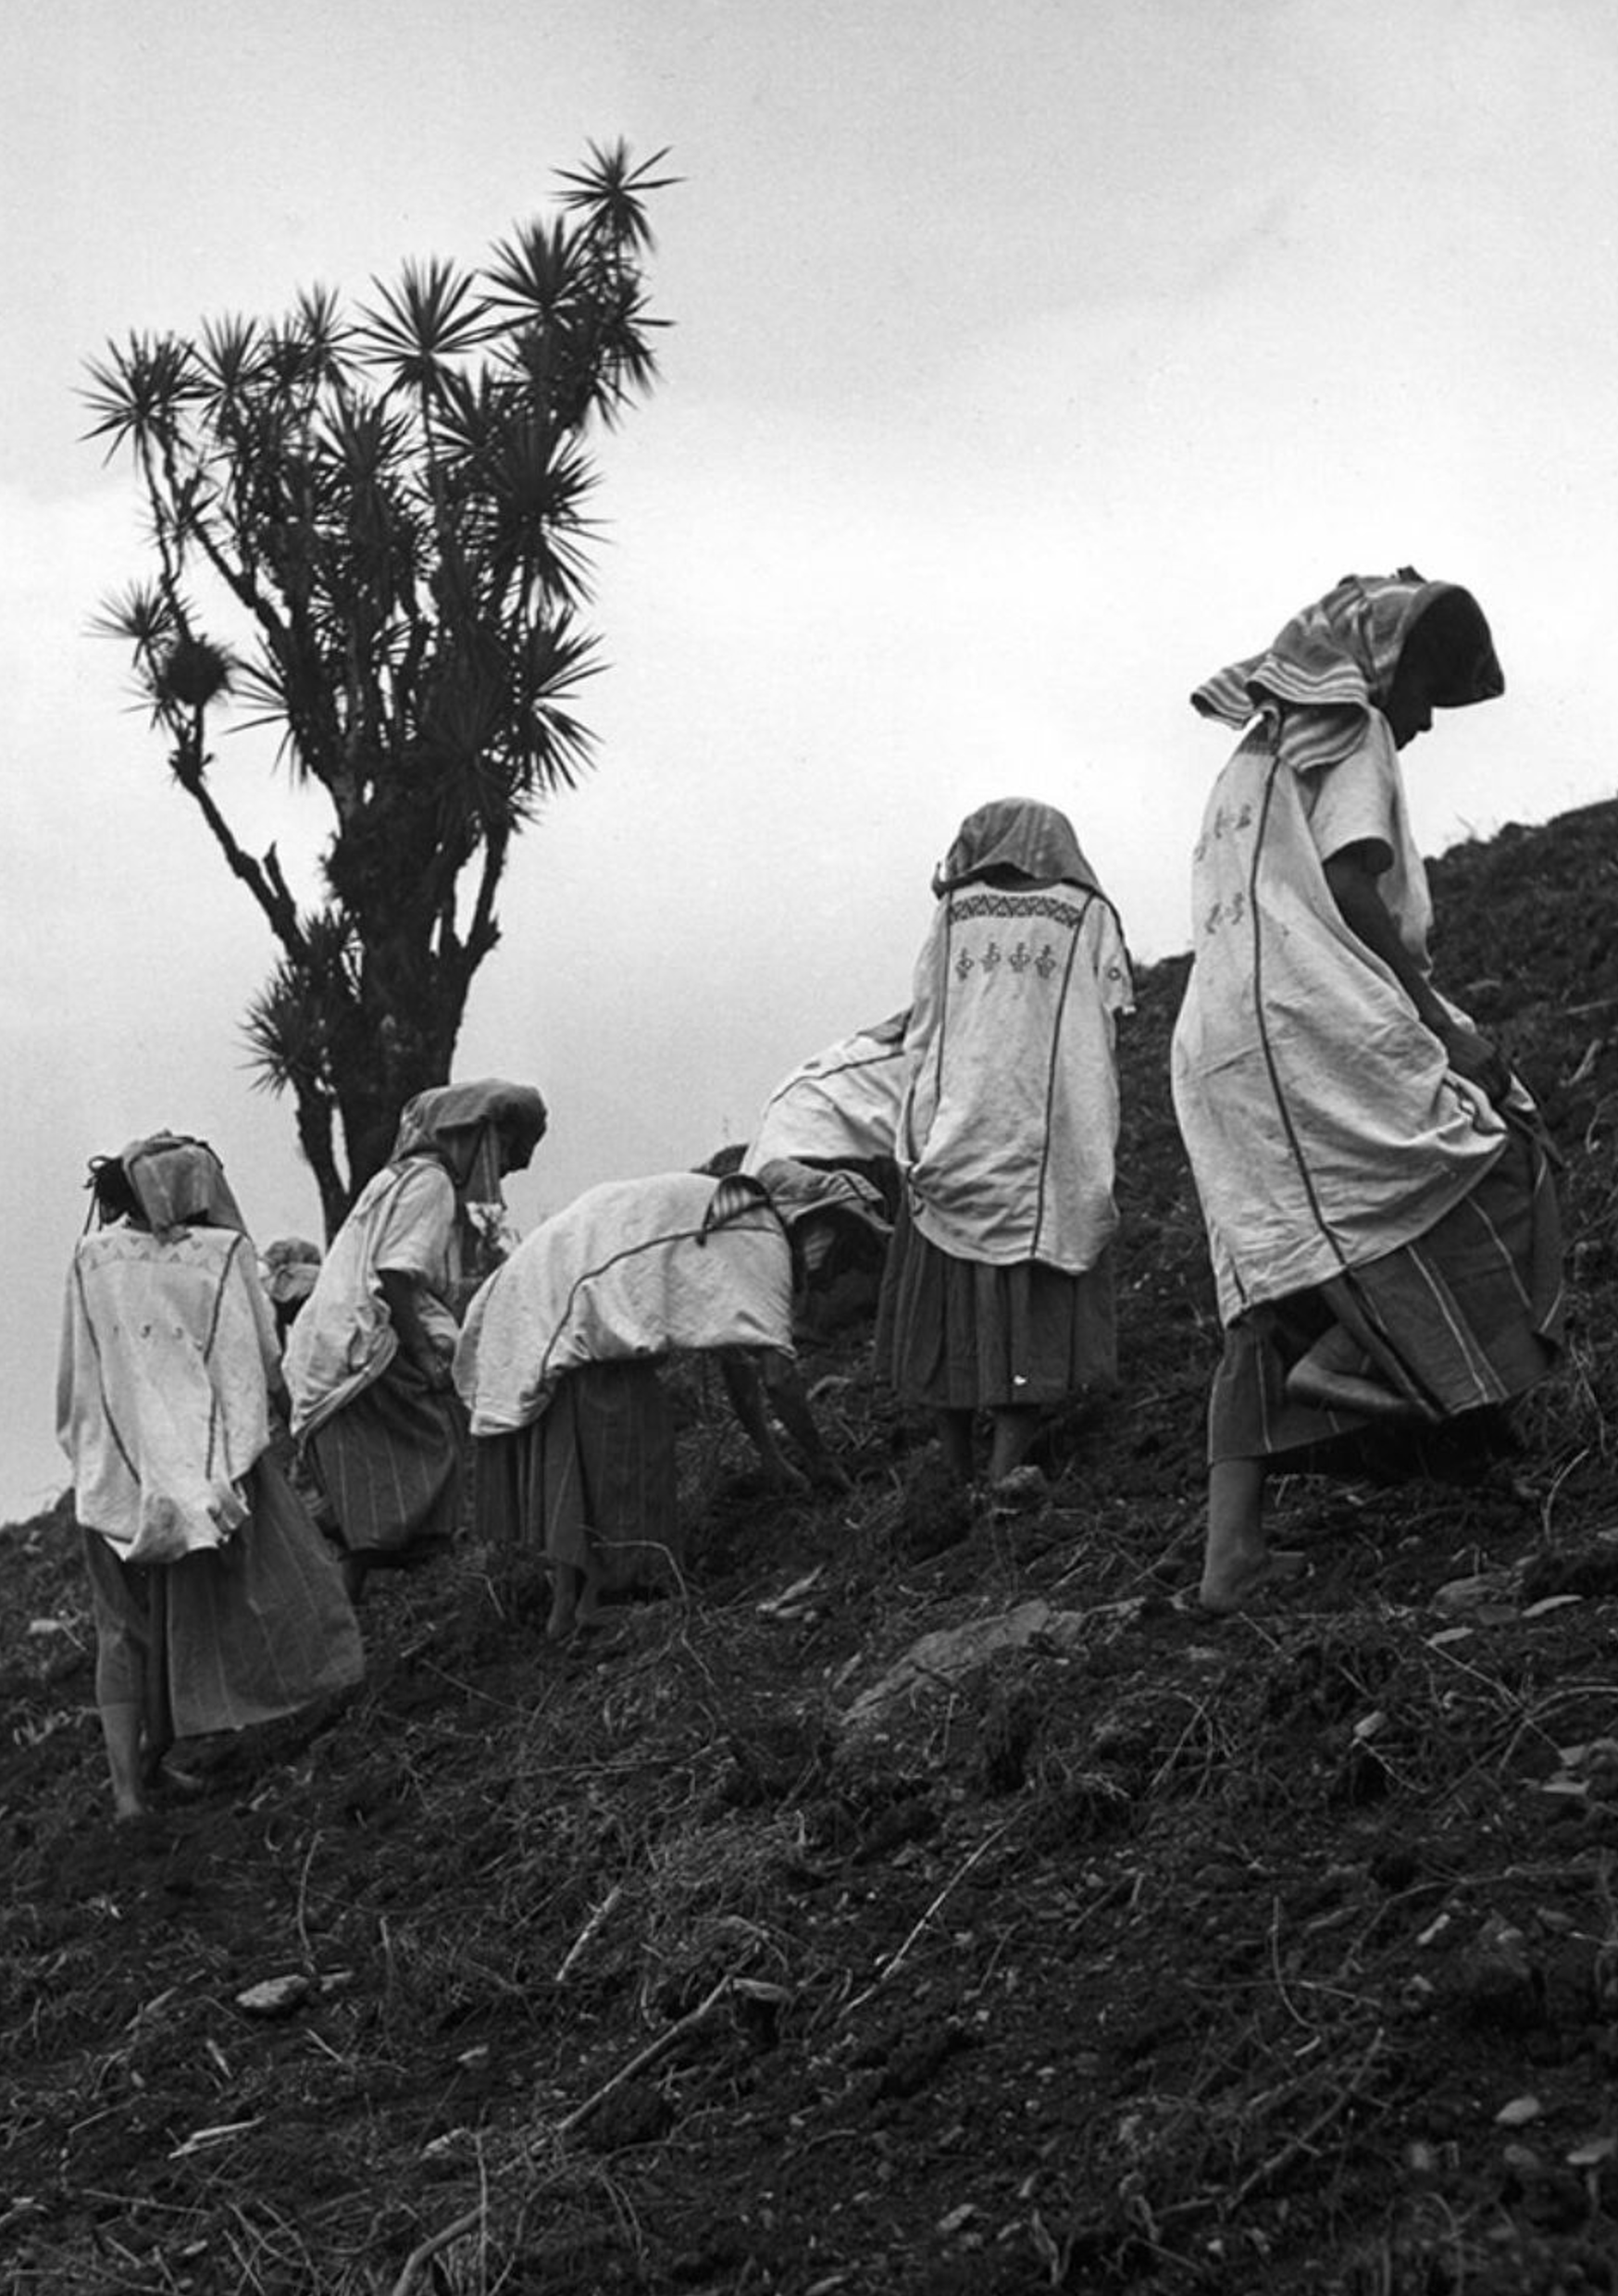
\includegraphics[height=\paperheight]{campesinas}};
	
	\node (ref) at (current page.north east) {};
	\draw (ref) node [purple,anchor=mid east,xshift=-1cm,yshift=-1.5cm,scale=4] {Rulfo};
	
	\node (ref) at (current page.south) {};
	\node[above = \baselineskip of ref] (rect) [purple,fill,minimum width=0.2cm,minimum height=1cm] {};
	\draw (rect) node [white,anchor=mid west,xshift=0.25cm,scale=2.5] {extraits};
	\draw (rect) node [white,anchor=mid east,xshift=-0.25cm,scale=2.5] {fragmentos};
\end{tikzpicture}

%\begin{tikzpicture}[remember picture,overlay]
%	
%	%\draw[white] (10,-13.5) node[scale=4,anchor=east] {Rulfo};
%	%\draw[white] (10,-13.5) node[scale=4,anchor=east] {\bf Rulfo};
%\end{tikzpicture}
%
%%\fontfamily{lmr}\selectfont
%
%\begin{tikzpicture}[remember picture,overlay]
%	%\fill[purple] (10,-13.5) rectangle (10+0.2,-13.5+1) node {};
%	
%\end{tikzpicture}
\end{document}